\section{Architektura systemu}
\subsection{Ogólny zarys architektury}
System wykonany będzie w~oparciu o~architekturę klient -- serwer. Rolę klientów pełnić będą komputery znajdujące się z~salonikach, bądź też komputer używany przez osobę zarządzającą siecią salonów. Rolę serwera pełnić będzie serwer aplikacji, oraz komunikujący się z~nim serwer bazy danych. W~każdym z~saloników, do komputera podłączona będzie kasa fiskalna, przeznaczona do prowadzenia sprzedaży oraz drukarka wykorzystywana do drukowania faktur dla klientów oraz raportów dla kierownika salonu.
\begin{figure}
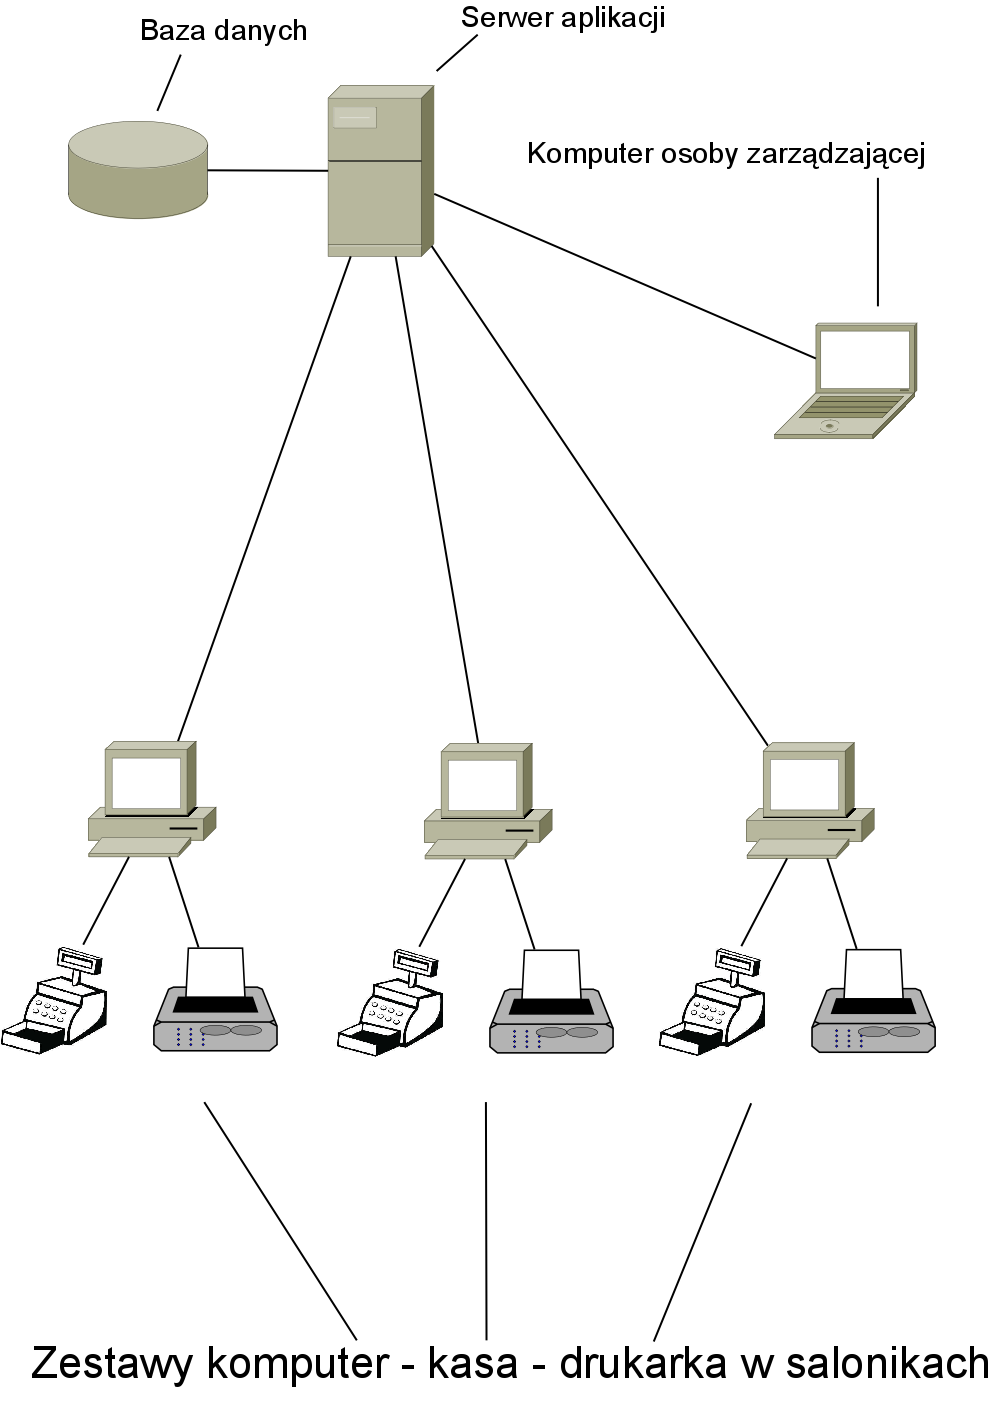
\includegraphics[width=1\textwidth]{gfx/architektura.png}
\caption{Ogólny zarys architektury systemu}
\end{figure}
\subsection{Platforma systemowa}
Zarówno serwer jak i~klient systemu napisane zostaną z~wykorzystaniem technologii Java 1.6. Komputery--klienty pracować będą pod kontrolą systemu operacyjnego Windows XP\texttrademark ,~natomiast serwer aplikacji uruchomiony będzie pod kontrolą systemu Linux. Baza danych wykorzystywana przez system działać będzie w~systemie PostreSQL, a~połączenie z~bazą będzie możliwe tylko z~serwera aplikacji.
\subsection{Komunikacja}
\subsubsection{Połączenie}
Każdy klient podłączać się będzie do serwera poprzez łącze internetowe dostępne w~saloniku (ADSL lub GPRS). Klient będzie podłączony do serwera co najmniej tak długo, jak długo trwać będzie praca salonu. Podłączenie do serwera możliwe będzie jedynie, gdy klient posiadać będzie odpowiedni identyfikator, zależny od salonika skojarzonego z~tym klientem oraz klucz, który będzie regularnie zmieniany bez ingerencji użytkownika podczas pracy systemu. Wszystkie próby (zarówno udane jak i~nie udane) serwer powinien odnotować w~swoich logach.
\subsubsection{Bezpieczeństwo}
Wszelka komunikacja pomiędzy serwerem, a~klientem odbywać się będzie za pośrednictwem szyfrowanego połączenia. Połączenie zestawiane będzie przy wykorzystaniu szyfru asymetrycznego, a~następnie wymieniony zostanie losowo wygenerowany klucz symetryczny, przy pomocy którego będzie się odbywało szyfrowanie i~deszyfrowanie przesyłanych danych.
\subsection{Kasa fiskalna}

\subsection{Dane techniczne kasy fiskalnej}
\begin{figure}
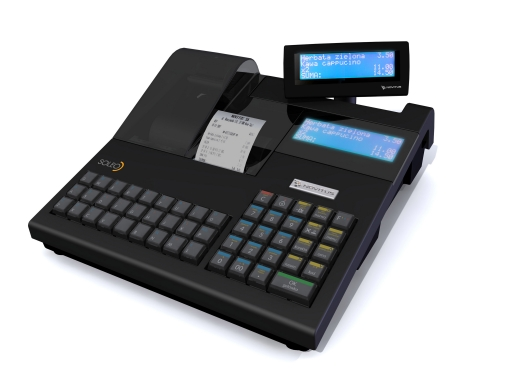
\includegraphics[width=1\textwidth]{gfx/SOLENO.jpg}
\caption{Kasa fiskalna SOLEO}
\end{figure}
\subsubsection{Typ kasy fiskalnej}
\begin{description}

\item Kasa fiskalna używana w~salonikach, to~kasa SOLEO\footnote{\href{http://www.novitus.pl/pl/cok/download/instrukcje-obslugi/instr_obslugi_soleo_v18.pdf} {Instrukcja obsługi kasy}}  firmy \href{http://www.novitus.pl/pl} {NOVITUS SA}. Kasa ta posiada następujące cechy:	
\begin{itemize}
\item Graficzne wyświetlacze obsługi i~klienta z~możliwością wyboru wielkości wyświetlanych znaków
\item Duża baza towarów: 7 000
\item Możliwość używania kodu porządkowego (2 kody na~towar)
\item Bufor On-line 500 pozycji sprzedaży
\item Identyfikacja 10~kasjerów
\item 8 wbudowanych stałych form płatności oraz dodatkowe 4~w~pełni definiowalne
\item 108 programowalnych klawiszy kodów lub funkcji (27 klawiszy x 4 poziomy)
\item Szerokość papieru 57 mm, 48 znaków w wierszu, prędkość druku 14 linii tekstu/s. (5,51 cm/s.)
\item Obsługiwane urządzenia: waga, skaner, PC, modem, terminal EFT
\item Obsługa waluty Euro
\item Wyszukiwanie towaru po nazwie i~możliwość wyboru towaru z~definiowalnych list
\item Łączność sieciowa poprzez modem
\end{itemize} 
\end{description}
\subsubsection{Połączenie z komputerem i czytnikiem kodów}
Kasa połączona jest z~komputerem poprzez port szeregowy COM. Do obsługi komunikacji używana jest, dostarczana przez producenta, biblioteka ze~sterownikiem w~technologii Active~X (wersja 3.4.2). Do kasy można podłączyć dowolny kompatybilny czytnik kodów kreskowych.
\subsection{Komunikacja pomiędzy bazą a kasą}
Kasa komunikuje się z~bazą danych za~pośrednictwem komputera. Komuter ten, ma za zadanie pobierać zmiany danych  w~bazie i~przekazać je do kasy. Zmianami tymi mogą, w~szczególności, być:
\begin{itemize}
\item Dodanie nowego towaru\footnote{Kasa, w odróżnieniu od bazy, identyfikuje towar z~jego kodem PLU, co~znaczy, że~zmiana w~towarze do~którego przypisane jest kilka kodów PLU, będzie przekazana do~kasy jako zmiana tylu towarów, ile jest tych kodów.}
\item Zmiana ceny
\item Usunięcie towaru
\item Nowe loginy, hasła użytkowników (sprzedawców)
\item Dostępność towaru 
\end{itemize} 
Komputer ma za zadanie także pobierać z~kasy, dane dotyczące sprzedaży, przetwarzać je, a~następnie przekazywać do~serwera. Dane te, to między innymi:
\begin{itemize}
\item Zalogowanie użytkownika (data)
\item Sprzedaż towaru
\item Wystawienie faktury VAT
\end{itemize} 
\subsection{Przykładowy opis działania systemu}
\subsubsection{Zmiana ceny towaru przez kierownika sieci}
Kierownik sieci uruchamia na swoim komputerze klienta. Klient podłącza się do serwera aplikacji. Następnie kierownik, korzystając ze swojego loginu oraz hasła loguje się do systemu. Korzystając z~interfejsu udostępnionego przez klienta, zmienia cenę towaru X. Informacja o~żądaniu zmiany towaru jest przesyłana do serwera, a~ten wprowadza poprawkę do bazy danych. Serwer sprawdza też, w~ofercie których saloników znajduje się towar o~zmienionej właśnie cenie. Następnie, do klientów odpowiadających tym salonikom, w~którym towar się znajduje, wysyłana jest informacja o~zmianie tej ceny. Jeżeli dany klient jest w~tej chwili nie osiągalny (nie jest podłączony do systemu, np. z~powodu awarii łącza w~saloniku), wiadomość o~zmianie ceny zostaje dodana do kolejki wiadomości przeznaczonych dla tego klienta. Klient w~momencie odebrania takiej informacji, pobiera z~serwera aktualną bazę informacji o~cenach i~produktach znajdujących się w~ofercie danego saloniku, a~następnie aktualne dane automatycznie wprowadzane są do kasy.
\subsubsection{Sprzedaż towaru w~saloniku}
Pracownik saloniku, rozpoczynając swoją zmianę, loguje się do systemu wykorzystując swój login i~hasło. W~momencie zatwierdzenia sprzedaży na kasie, informacja o~sprzedanych towarach wysyłana jest z~kasy do klienta. Klient propaguje tą informację do serwera dołączając wzbogacając ją dodatkowo o~informacje na temat identyfikatora sprzedającego, czy czasu sprzedaży.